\documentclass[tikz]{standalone}% 'crop' is the default for v1.0, before it was 'preview'
\usepackage{tikz}
\usepackage{pgfplots}
\usepackage{amsmath}

\usepgfplotslibrary{colormaps}
\pgfplotsset{compat=1.18}
%\usetikzlibrary{...}% tikz package already loaded by 'tikz' option
\begin{document}


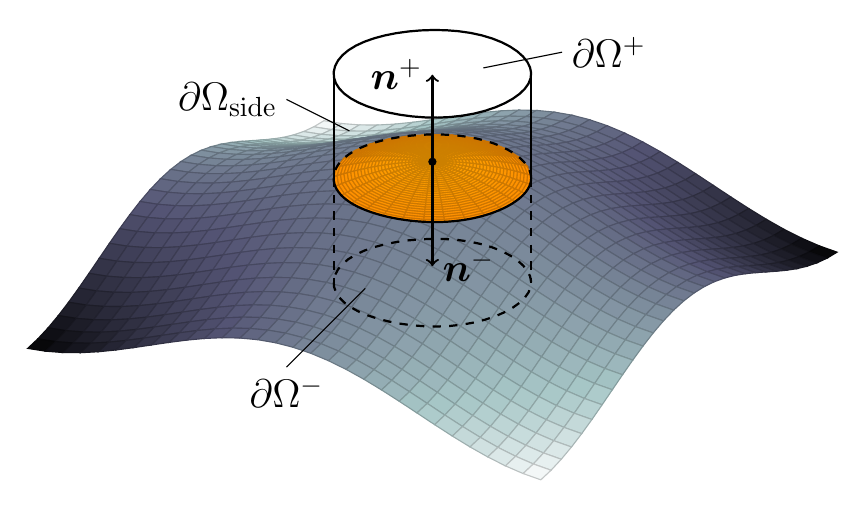
\begin{tikzpicture}[font=\Large]
\begin{axis}[
    hide axis,
    scale=2,
    view={120}{40},
    xmin=-4,xmax=4,
    ymin=-4,ymax=4,
    zmin=-2,zmax=10,
    trig format plots=rad,
  ]
    % Draw big surface
    \addplot3 [ surf, colormap/bone, domain=-3:3, domain y=-3:3, samples=30, samples y=30, variable=\u, variable y=\v, point meta=u*v]
    ( {u}, {v}, {cos(u) + cos(v)} );

    % Draw small surface
    \addplot3 [ surf, colormap/hot2, domain=0:2*pi, domain y=0:1, samples=30, samples y=30, variable=\u, variable y=\v]
    ( {v*cos(u)}, {v*sin(u)}, {cos(v*cos(u)) + cos(v*sin(u))} );
    \pgfmathsetmacro{\vartangent}{2/3} % Define the variable here

    % Middle ellipse
    \addplot3[black, thick, variable=\t, domain=\vartangent-1:\vartangent, samples=50, samples y=1] ( {cos(pi*t)}, {sin(pi*t)}, {cos(cos(pi*t)) + cos(sin(pi*t))});
    \addplot3[black, thick, dashed, variable=\t, domain=\vartangent:\vartangent+1, samples=50, samples y=1] ( {cos(pi*t)}, {sin(pi*t)}, {cos(cos(pi*t)) + cos(sin(pi*t))});

    % Top ellipse
    \addplot3[black, thick, variable=\t, domain=-1:1, samples=50, samples y=1] ( {cos(pi*t)}, {sin(pi*t)}, {cos(cos(pi*t)) + cos(sin(pi*t)) + 3});

    % Bottom ellipse
    \addplot3[black, thick, dashed, variable=\t, domain=-1:1, samples=50, samples y=1] ( {cos(pi*t)}, {sin(pi*t)}, {cos(cos(pi*t)) + cos(sin(pi*t)) - 3});


    \addplot3[black, thick, variable=\t, domain=0:3, samples y=1] ( {cos(pi*\vartangent)}, {sin(pi*\vartangent)}, {cos(cos(pi*\vartangent)) + cos(sin(pi*\vartangent)) + t});
    \addplot3[black, thick, variable=\t, domain=0:3, samples y=1] ( {-cos(pi*\vartangent)}, {-sin(pi*\vartangent)}, {cos(-cos(pi*\vartangent)) + cos(-sin(pi*\vartangent)) + t});
    \addplot3[black, thick, dashed, variable=\t, domain=0:-3, samples y=1] ( {cos(pi*\vartangent)}, {sin(pi*\vartangent)}, {cos(cos(pi*\vartangent)) + cos(sin(pi*\vartangent)) + t});
    \addplot3[black, thick, dashed, variable=\t, domain=0:-3, samples y=1] ( {-cos(pi*\vartangent)}, {-sin(pi*\vartangent)}, {cos(-cos(pi*\vartangent)) + cos(-sin(pi*\vartangent)) + t});
    \draw[->, thick, black] (axis cs:0,0,2) -- (axis cs: 0,0,4.5) node[left] {$\boldsymbol{n}^+$}; 
    \draw[->, thick, black] (axis cs:0,0,2) -- (axis cs: 0,0,-1) node[right] {$\boldsymbol{n}^-$};
    \node[circle,fill=black,inner sep=0pt,minimum size=3pt] at (axis cs: 0,0,2) {}; 
\end{axis}
  
\draw[thin, black] (8.5,6.2)  node[right] {$\partial \Omega^+$} -- (7.5,6);
\draw[thin, black] (5,2.2)  node[below] {$\partial \Omega^-$} -- (6,3.2);
\draw[thin, black] (5,5.6)  node[left] {$\partial \Omega_\mathrm{side}$} -- (5.8,5.2);


\end{tikzpicture}
\end{document}